\begin{figure}[ht]
\centering
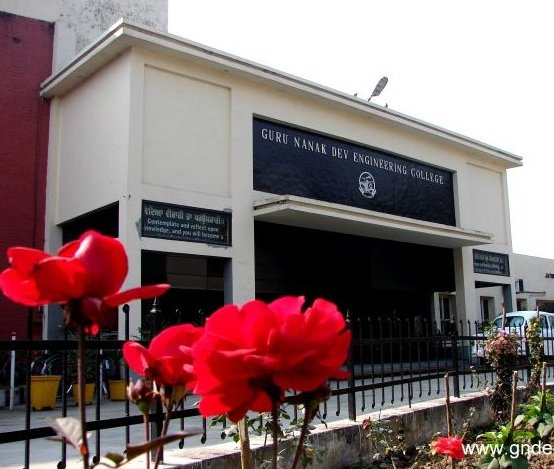
\includegraphics[scale=0.7]{images/gndec.jpg}
\caption{Guru Nanak Dev Engineering College}
\end{figure}
\hspace{-1.7em} I had my Six Month Industrial Training at APTECH Ludhiana. Guru Nanak Dev Engineering College was established by the Nankana
Sahib Education Trust Ludhiana. The Nankana Sahib Education Trust i.e NSET
was founded in memory of the most sacred temple of Sri Nankana Sahib, birth place
of Sri Guru Nanak Dev Ji. With the mission of Removal of Economic Backwardness
through Technology Shiromani Gurudwara Parbandhak Committee i.e SGPC started a
Poly technical was started in 1953 and Guru Nanak Dev Engineering College was established in 1956.\\\\
NSET resolved to uplift Rural areas by admitting 70\% 
of students from these rural
areas ever year. This commitment was made to nation on 8th April, 1956, the day
foundation stone of the college building was laid by Dr. Rajendra Prasad Ji, the First
President of India. The College is now ISO 9001:2000 certified.\\\\
Guru Nanak Dev Engineering College campus is spread over 88 acres of prime land
about 5 Km s from Bus Stand and 8 Km s from Ludhiana Railway Station on Ludhiana-Malerkotla Road. The college campus is well planned with beautifully laid out tree plantation, pathways, flowerbeds besides the well maintained sprawling lawns all around. It
has beautiful building for College,Hostels,Swimming Pool,Sports and Gymnasium Hall
Complex, Gurudwara Sahib, Bank, Dispensary, Post Office etc. There are two hostels
for boys and one for girls with total accommodation of about 550 students. The main
goal of this institute is:\\\\
\begin{itemize}
\item To build and promote teams of experts in the upcoming specialisations.
\item To promote quality research and undertake research projects keeping in view their
relevance to needs and requirements of technology in local industry.
\item To achieve total financial independence.
\item To start online transfer of knowledge in appropriate technology by means of establishing multipurpose resource centres.
\end{itemize}
\section{APTECH Ludhiana}
My Six Month Industrial Training was done by me at APTECH Ludhiana under the guidance of Mrs. Ritu Verma Centre Head Aptech Ludhiana. 

\begin{figure}[ht]
\centering
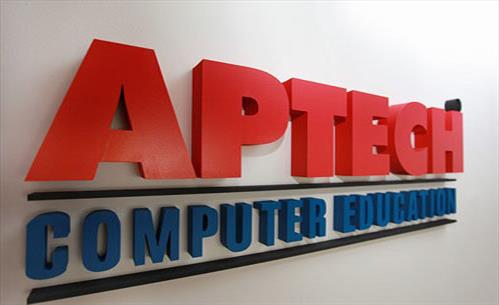
\includegraphics[scale=0.9]{images/Aptech.jpg}
\caption{Aptech Computer Education}
\end{figure} 

\noindent Aptech Computer Education is a premier IT
education Institute. Established in 1986, Aptech is a
pioneer in IT software \& hardware training. The Institute has successfully trained more than 70
lakh (7 million) students through its wide network
of education centres located in over 40 countries.\\

\noindent Aptech offers a variety of courses - technology
courses for IT students, career programs for students
wanting to enter the IT sector, certification courses
for IT professionals to enhance their career and basic
IT programs for school students, housewives/senior
citizens etc. Class timings are such that even working people can attend courses as per their convenience.\\

\noindent Aptech Computer Education has alliances with three of the leading computer technology companies to offer courses that are globally recognized. These tie-ups enable us to provide our students official curriculum of international standards. In addition, students also receive discounts on certification exams and a participation certificate by the respective global alliance partners. Aptech Computer Education prepares students to be a part of this growing industry through its
courses, partnerships with technology companies like Microsoft, Red Hat, Oracle \& various placement assistance activities.\\\\


THE ACADEMY OFFERS:\\
\begin{itemize}
\item World class quality of education.
\item A wide range of courses.
\item Benefits through partnerships with leading technology companies such as Microsoft, Red Hat, Java \& Oracle.
\item Job placement assistance after successful completion of career courses
\end{itemize}

